%==================================================%
% Basic setup starts here
%==================================================%
\documentclass[12pt, letterpaper]{amsart} % this will automatically load amsmath and amsthm packages
\usepackage{amsfonts}
\usepackage{amscd} % a CD environment for commutative rectangular diagram
\usepackage{mathtools} % for \shortintertext
\usepackage[utf8]{inputenc} % encoding method
\usepackage[mathscr]{eucal} % eucal calligraphy, mathsrc = use \mathcal
\usepackage{indentfirst} % indent first line of all sections
\usepackage{graphicx} % extension of graphics, options for \includegrahpicx
\usepackage{pict2e} % new implementation of the picture environment, which allows programming pictures directly LaTeX
\usepackage{epic} % add some command to the picture environment
\usepackage[margin=2.9cm]{geometry} % customize page layout

\usepackage{glossaries}
\usepackage{hyperref}

\usepackage[utf8]{inputenc}
\usepackage{amsmath,amssymb, amsthm}
\usepackage{enumitem}
\newlength{\mylen}
\setlength{\mylen}{0.5ex}
\renewcommand\labelitemi{\raisebox{0.5ex}{\tiny$\bullet$}}

%==================================================%
% Additional setup ends here
%==================================================%
% Additional package used for relevant article
\usepackage{physics} % partial derivative \pdv
\usepackage{cleveref} % automatically add eq in referencing
\usepackage{cancel}
\usepackage{tikz}
\usepackage{graphicx}
\graphicspath{ {images/} }

% SELF-DEFINED THEOREM using amsthm package
\newtheorem{Th}{Theorem}[section]
\numberwithin{equation}{section}
\newtheorem{Def}[Th]{Definition}




%==================================================%
% Glossary
%==================================================%
%==================================================%
% Document starts here
% ==================================================%
\author{Author(s): \\ \\ Kin Chang \\ 
Lin Li\\Amir Omidfar}
\title{Lab 3 and 4 Report}
\begin{document}
\maketitle
\pagebreak
\tableofcontents
\pagebreak
\section*{Lab Overview:}
This lab derives a mathematical input-output model of the system dynamics based on a model of sensor and actuator responses for a two wheel car. Using this model in computational environment it would then create a state estimator for the location of the car in a 4 wall bounding open space. State estimator follows extended Kalman filter procedure to derive required results.



\begin{figure}[h!]
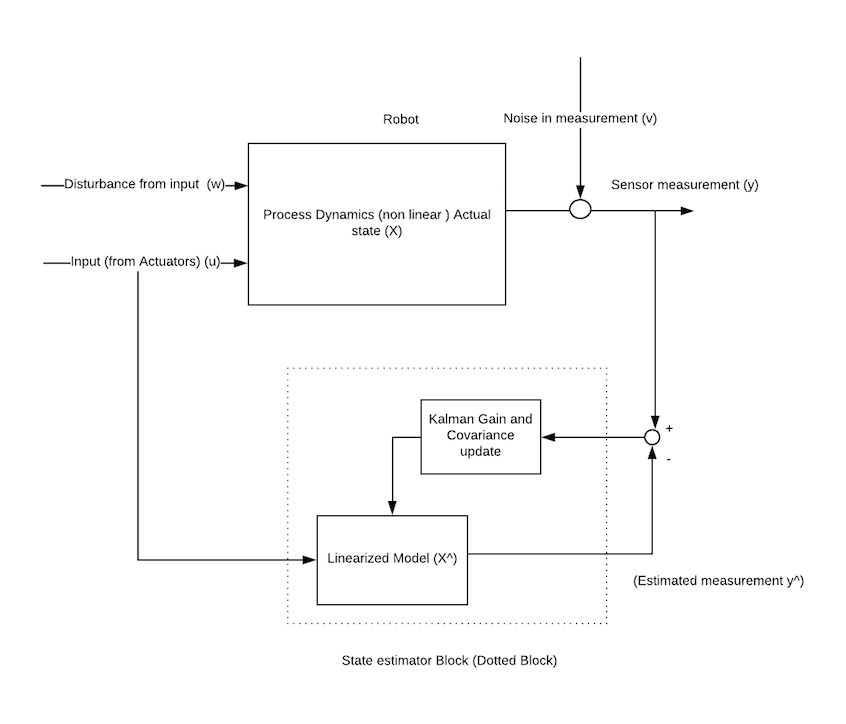
\includegraphics[width=110mm]{fig_1.png}
\caption{System Block Diagram}
\label{fig:figure1}
\end{figure}

Kalman filter would provide a linearized model of the robot.The point of this procedure is to minimize the difference between actual measurements and the filter approximations $(y-y\hat{})$ therefore with each iteration through the loop state of robot can be calculated with great accuracy.   
\\
\newpage
\section{Symbols}
Here is the list of all symbols we used for deriving Kalman filter in order to build state estimator:
\\
\begin{tabular}{c p{1\textwidth}}
  $L_x$ & length of the box  \\
  $L_y$ & width of the box \\
  $W$ & distance between rotating center and sensors center \\
  $C_v$ & coefficient, distance traveled by the wheel per unit of delay time \\
  $C_r$ & coefficient, body orientation changed by the wheel per unit of delay time \\
  $l_x$ & first range sensor reading (located on front of the car) \\
  $l_y$ & second range sensor reading (located on right side of the car) \\
  $\alpha$ & MPU angle measurement \\
  $r_x$ & absolute x coordinate of the car \\
  $r_y$ & absolute y coordinate of the car \\
  $\theta$ & absolute orientation of the car \\
  $\tau_L$ & Servo input: delay time of the left wheel \\
  $\tau_R$ & Servo input: delay time of the right wheel \\
  $\theta_{tht}$ & top half threshold angle \\
  $\theta_{thb}$ & bottom half threshold angle \\
  $\theta_{thr}$ & bottom right threshold angle \\
  $\theta_{thl}$ & bottom left threshold angle \\
  $\epsilon_{str}$ & picking variable, 1 if going straight line, 0 otherwise \\
  $w_t$ & process noise \\
  $v_t$ & measurement noise
\end{tabular}\\
\\ \\ \\ \\ \\ \\

\newpage
\section{Assumption}
For the sake of simplicity, we have the following assumption in the derivation below
\begin{enumerate}
\item $\theta$ takes value only (-90, 90)
\item $\tau_L$ and $\tau_R$ has the same magnitude, opposite sign if turning, otherwise same sign 
\item $\theta = \alpha$ assuming we have the the MPU calibrated at the 0 point
\end{enumerate}  



\begin{align*}
  \intertext{State}
  x = 
  \begin{bmatrix}
    r_x \\
    r_y \\
    \theta 
  \end{bmatrix} \\
  \intertext{Sensor Measurements}
  y = 
  \begin{bmatrix}
    l_x \\
    l_y \\
    \alpha
  \end{bmatrix} \\
  \intertext{Input}
  u = 
  \begin{bmatrix}
    \tau_L \\
    \tau_R
  \end{bmatrix} \\  
\end{align*}

\section{Sensor Measurement}
As shown in the picture below, $\theta$ is the angle the head of the car would have with respect to the direction of $L_x$. In order to do the calculations required there are four more threshold angles defined as tht (top), thb (bottom), thr (right) and thl(left). 
\begin{figure}[h!]
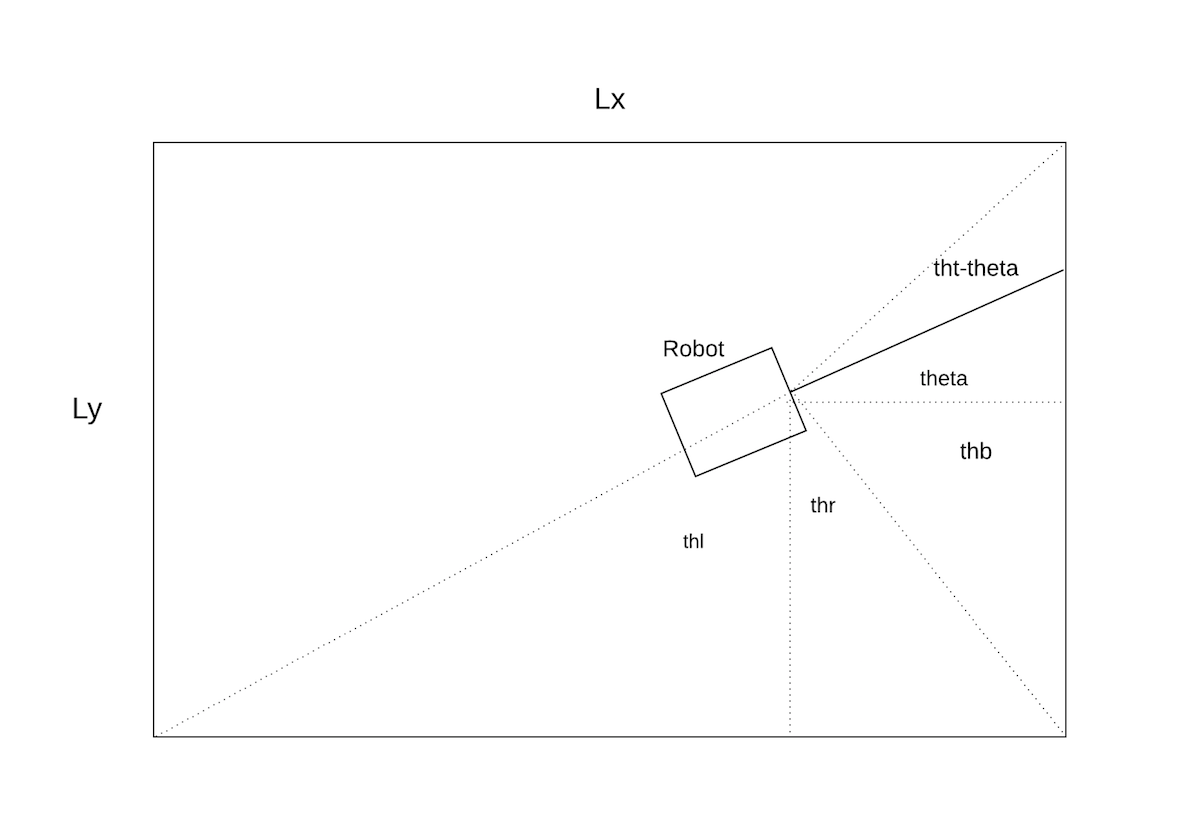
\includegraphics[width=110mm]{fig_2.png}
\caption{Threshold angles and theta ($\theta$)}
\label{fig:figure2}
\end{figure}
\\
\\
These angles are then used to find a function such that $y = h(x)$ \\
Threshold angles can be shown using trigonometry relationships:
\begin{align*}
  \theta_{tht} &= \tan^{-1}(\frac{L_y - r_y}{L_x - r_x}) \\
  \theta_{thb} &= \tan^{-1}(\frac{r_y}{L_x - r_x}) \\
  \theta_{thr} &= \tan^{-1}(\frac{L_x-r_x}{r_y}) \\
  \theta_{thl} &= \tan^{-1}(\frac{r_x}{r_y})
\end{align*}











Under mentioned assumption, the expression for $l_x$ (front range sensor reading) varies based on below four cases:
\begin{align*}
  l_x = \frac{L_x - r_x}{\cos \theta} \quad ,\quad 0 < \theta < \theta_{tht} \\
  l_x = \frac{L_y - r_y}{\sin \theta} \qquad  \theta > \theta_{tht} \\
  l_x = \frac{L_x - r_x}{\cos \theta} \quad \theta < 0, |\theta| < |\theta_{thb}| \\
  l_x = \frac{r_y}{\sin|\theta|} \quad \theta < 0, |\theta| > \theta_{thb}
\end{align*}
the expression for $l_y$ (right side sensor reading) varies under these four cases:
\begin{align*}
  l_y = \frac{r_y}{\cos |\theta|} \quad  ,\quad 0 < \theta < \theta_{thr} \\
  l_y = \frac{L_x - r_x}{\sin |\theta|} \qquad \theta > \theta_{thr} \\
  l_y = \frac{r_y}{\cos |\theta|} \quad \theta < 0, |\theta| < \theta_{thl} \\
  l_y = \frac{r_x}{\sin |\theta|} \quad \theta < 0, |\theta| > \theta_{thl}
\end{align*}
The derived expression for $\alpha = \theta$ doesn't change under the mentioned assumption. \par
\newpage
To summarize, there are total of 8 cases as indicated below:
\\
\begin{align*}
  \intertext{$\theta \geq 0, |\theta| < \theta_{tht}, |\theta| < \theta_{thr}$}
  y = 
  \begin{bmatrix}
    \frac{L_x - r_x}{\cos |\theta|} \\
    \frac{r_y}{\cos |\theta|} \\
    \alpha = \theta
  \end{bmatrix}
  \intertext{$\theta>0, |\theta| < \theta_{tht}, |\theta| > \theta_{thr}$}
  y = 
  \begin{bmatrix}
    \frac{L_x - r_x}{\cos |\theta|} \\
    \frac{L_x - r_x}{\sin |\theta|} \\
    \alpha = \theta
  \end{bmatrix}
  \intertext{$\theta>0, |\theta| > \theta_{tht}, |\theta| < \theta_{thr}$}
  y = 
  \begin{bmatrix}
    \frac{L_y - r_y}{\sin |\theta|} \\    
    \frac{r_y}{\cos |\theta|} \\
    \alpha = \theta
  \end{bmatrix}
  \intertext{$\theta>0, |\theta| > \theta_{tht}, |\theta| > \theta_{thr}$}
  y = 
  \begin{bmatrix}
    \frac{L_y - r_y}{\sin |\theta|} \\
    \frac{L_x - r_x}{\sin |\theta|} \\
    \alpha = \theta
  \end{bmatrix}
  %% \theta < 0
  \intertext{$\theta<0, |\theta| < \theta_{thb}, |\theta| < \theta_{thl}$}
  y = 
  \begin{bmatrix}
    \frac{L_x - r_x}{\cos |\theta|} \\
    \frac{r_y}{\cos |\theta|} \\
    \alpha = \theta
  \end{bmatrix}
  \intertext{$\theta<0, |\theta| < \theta_{thb}, |\theta| > \theta_{thl}$}
  y = 
  \begin{bmatrix}
    \frac{L_x - r_x}{\cos |\theta|} \\
    \frac{r_x}{\sin |\theta|} \\
    \alpha = \theta
  \end{bmatrix}
  \intertext{$\theta<0, |\theta| > \theta_{thb}, |\theta| < \theta_{thl}$}
  y = 
  \begin{bmatrix}
    \frac{r_y}{\sin |\theta|} \\    
    \frac{r_y}{\cos |\theta|} \\
    \alpha = \theta
  \end{bmatrix}
  \intertext{$\theta<0, |\theta| > \theta_{thb}, |\theta| > \theta_{thl}$}
  y = 
  \begin{bmatrix}
    \frac{r_y}{\sin |\theta|} \\        
    \frac{r_x}{\sin |\theta|} \\
    \alpha = \theta
  \end{bmatrix}  
\end{align*}
\\
\\
Now in order to obtain the model shown in Figure 1, all eight cases have to be linearized in order to derive matrix H where: $y = H x$. As for demonstratation purposes the linearization of case one where $\theta >0, |\theta| < \theta_{tht}, |\theta| < \theta_{thr}$, is shown:
\begin{align*}
  l_x &= \frac{L_x - r_x}{\cos \theta} \\
  l_y &= \frac{r_y}{\cos \theta} \\
  \intertext{Linearization around $l_{x0}, l_{y0}, \alpha_{0} = h(r_{x0}, r_{y0}, \theta_0)$}
  l_x &= l_{x0} + \frac{-1}{\cos \theta_0} (r_x - r_{x0}) + \frac{(L_x - r_{x0})\sin(\theta_0)}{(\cos{\theta_0})^2} (\theta - \theta_0) \\
  l_y &= l_{y0} + \frac{1}{\cos \theta_0}(r_y - r_{y0}) + \frac{r_{y0} \sin(\theta_0)}{(\cos \theta_0)^2} (\theta - \theta_0) \\
  l_x &= \frac{-1}{\cos \theta_0} r_x + \frac{(L_x - r_{x0})\sin(\theta_0)}{(\cos{\theta_0})^2} \theta + [\frac{r_{x0}}{\cos \theta_0} - \frac{(L_x - r_{x0})\sin(\theta_0)}{(\cos{\theta_0})^2}\theta_0 + l_{x0}] \\
  l_y &= \frac{1}{\cos \theta_0}r_y + \frac{r_{y0} \sin(\theta_0)}{(\cos \theta_0)^2} \theta + [\frac{-r_{y0}}{\cos \theta_0} - \frac{r_{y0} \sin(\theta_0)}{(\cos \theta_0)^2} \theta_0 + l_{y0}]
\end{align*}
In matrix form, the complete form for this case is
\begin{align*}
  y =
  \begin{bmatrix}
    \frac{-1}{\cos \theta_0} & 0 & \frac{(L_x - r_{x0})\sin(\theta_0)}{(\cos{\theta_0})^2} \\
    0 & \frac{1}{\cos \theta_0} & \frac{r_{y0} \sin(\theta_0)}{(\cos \theta_0)^2} \\
    0 & 0 & 1
  \end{bmatrix}
            \begin{bmatrix}
              r_x \\
              r_y \\
              \theta
            \end{bmatrix}
            +
            \begin{bmatrix}
              \frac{r_{x0}}{\cos \theta_0} - \frac{(L_x - r_{x0})\sin(\theta_0)}{(\cos{\theta_0})^2}\theta_0 + l_{x0} \\
              \frac{-r_{y0}}{\cos \theta_0} - \frac{r_{y0} \sin(\theta_0)}{(\cos \theta_0)^2} \theta_0 + l_{y0} \\
              0
            \end{bmatrix}
\end{align*}

\newpage
\section{Complete Case Analysis}
\begin{align*}
  \intertext{$\theta \geq 0, |\theta| < \theta_{tht}, |\theta| < \theta_{thr}$}
  H &= 
  \begin{bmatrix}
    \frac{-1}{\cos \theta_0} & 0 & \frac{(L_x - r_{x0})\sin(\theta_0)}{(\cos{\theta_0})^2} \\
    0 & \frac{1}{\cos \theta_0} & \frac{r_{y0} \sin(\theta_0)}{(\cos \theta_0)^2} \\
    0 & 0 & 1
  \end{bmatrix}
            \quad
            C =
            \begin{bmatrix}
              \frac{r_{x0}}{\cos \theta_0} - \frac{(L_x - r_{x0})\sin(\theta_0)}{(\cos{\theta_0})^2}\theta_0 + l_{x0} \\
              \frac{-r_{y0}}{\cos \theta_0} - \frac{r_{y0} \sin(\theta_0)}{(\cos \theta_0)^2} \theta_0 + l_{y0} \\
              0
            \end{bmatrix}            
  \intertext{$\theta \geq 0, |\theta| < \theta_{tht}, |\theta| > \theta_{thr}$}
  H &= 
  \begin{bmatrix}
    \frac{-1}{\cos \theta_0} & 0 & \frac{(L_x - r_{x0})\sin(\theta_0)}{(\cos{\theta_0})^2} \\
    \frac{-1}{\sin |\theta_0|} & 0 & -\frac{\theta_0}{|\theta_0|}\frac{L_x - r_{x0} \cos(\theta_0)}{(\sin |\theta_0|)^2} \\
    0 & 0 & 1
  \end{bmatrix}
            \quad
            C =
            \begin{bmatrix}
              \frac{r_{x0}}{\cos \theta_0} - \frac{(L_x - r_{x0})\sin(\theta_0)}{(\cos{\theta_0})^2}\theta_0 + l_{x0} \\
              \frac{r_{x0}}{\sin |\theta_0|} + \frac{(L_x - r_{x0}) \cos(\theta_0)}{(\sin |\theta_0|)^2} |\theta_0| + l_{y0} \\
              0
            \end{bmatrix}            
  \intertext{$\theta>0, |\theta| > \theta_{tht}, |\theta| < \theta_{thr}$}
  H &= 
  \begin{bmatrix}
    0 & \frac{-1}{\sin |\theta_0|} & -\frac{\theta_0}{|\theta_0|}\frac{L_y - r_{y0} \cos(\theta_0)}{(\sin |\theta_0|)^2} \\    
    0 & \frac{1}{\cos \theta_0} & \frac{r_{y0} \sin(\theta_0)}{(\cos \theta_0)^2} \\
    0 & 0 & 1
  \end{bmatrix}
            \quad
            C =
            \begin{bmatrix}
              \frac{r_{y0}}{\sin |\theta_0|} + \frac{(L_y - r_{y0}) \cos(\theta_0)}{(\sin |\theta_0|)^2} |\theta_0| + l_{x0} \\              
              \frac{-r_{y0}}{\cos \theta_0} - \frac{r_{y0} \sin(\theta_0)}{(\cos \theta_0)^2} \theta_0 + l_{y0} \\
              0
            \end{bmatrix}              
  \intertext{$\theta>0, |\theta| > \theta_{tht}, |\theta| > \theta_{thr}$}
  H &= 
  \begin{bmatrix}
    0 & \frac{-1}{\sin |\theta_0|} & -\frac{\theta_0}{|\theta_0|}\frac{L_y - r_{y0} \cos(\theta_0)}{(\sin |\theta_0|)^2} \\
    \frac{-1}{\sin |\theta_0|} & 0 & -\frac{\theta_0}{|\theta_0|}\frac{L_x - r_{x0} \cos(\theta_0)}{(\sin |\theta_0|)^2} \\    
    0 & 0 & 1
  \end{bmatrix}
            \quad
            C =
            \begin{bmatrix}
              \frac{r_{y0}}{\sin |\theta_0|} + \frac{(L_y - r_{y0}) \cos(\theta_0)}{(\sin |\theta_0|)^2} |\theta_0| + l_{x0} \\
              \frac{r_{x0}}{\sin |\theta_0|} + \frac{(L_x - r_{x0}) \cos(\theta_0)}{(\sin |\theta_0|)^2} |\theta_0| + l_{y0} \\              
              0
            \end{bmatrix}                
  %% \theta < 0
  \intertext{$\theta<0, |\theta| < \theta_{thb}, |\theta| < \theta_{thl}$}
  H &= 
  \begin{bmatrix}
    \frac{-1}{\cos \theta_0} & 0 & \frac{(L_x - r_{x0})\sin(\theta_0)}{(\cos{\theta_0})^2} \\
    0 & \frac{1}{\cos \theta_0} & \frac{r_{y0} \sin(\theta_0)}{(\cos \theta_0)^2} \\
    0 & 0 & 1
  \end{bmatrix}
            \quad
            C =
            \begin{bmatrix}
              \frac{r_{x0}}{\cos \theta_0} - \frac{(L_x - r_{x0})\sin(\theta_0)}{(\cos{\theta_0})^2}\theta_0 + l_{x0} \\
              \frac{-r_{y0}}{\cos \theta_0} - \frac{r_{y0} \sin(\theta_0)}{(\cos \theta_0)^2} \theta_0 + l_{y0} \\
              0
            \end{bmatrix}              
  \intertext{$\theta<0, |\theta| < \theta_{thb}, |\theta| > \theta_{thl}$}
  H &= 
  \begin{bmatrix}
    \frac{-1}{\cos \theta_0} & 0 & \frac{(L_x - r_{x0})\sin(\theta_0)}{(\cos{\theta_0})^2} \\
    \frac{1}{\sin |\theta_0|} & 0 & -\frac{\theta_0}{|\theta_0|}\frac{r_{x0} \cos(\theta_0)}{(\sin |\theta_0|)^2} \\
    0 & 0 & 1
  \end{bmatrix}
            \quad
            C =
            \begin{bmatrix}
              \frac{r_{x0}}{\cos \theta_0} - \frac{(L_x - r_{x0})\sin(\theta_0)}{(\cos{\theta_0})^2}\theta_0 + l_{x0} \\
              \frac{-r_{x0}}{\sin |\theta_0|} + \frac{r_{x0} \cos(\theta_0)}{(\sin |\theta_0|)^2} |\theta_0| + l_{y0} \\
              0
            \end{bmatrix}              
  \intertext{$\theta<0, |\theta| > \theta_{thb}, |\theta| < \theta_{thl}$}
  H &= 
  \begin{bmatrix}
    0 & \frac{1}{\sin |\theta_0|} & -\frac{\theta_0}{|\theta_0|}\frac{r_{y0} \cos(\theta_0)}{(\sin |\theta_0|)^2} \\    
    0 & \frac{1}{\cos \theta_0} & \frac{r_{y0} \sin(\theta_0)}{(\cos \theta_0)^2} \\
    0 & 0 & 1
  \end{bmatrix}
            \quad
            C =
            \begin{bmatrix}
              -\frac{r_{y0}}{\sin |\theta_0|} + \frac{r_{y0} \cos(\theta_0)}{(\sin |\theta_0|)^2} |\theta_0| + l_{x0} \\              
              \frac{-r_{y0}}{\cos \theta_0} - \frac{r_{y0} \sin(\theta_0)}{(\cos \theta_0)^2} \theta_0 + l_{y0} \\
              0
            \end{bmatrix}                
  \intertext{$\theta<0, |\theta| > \theta_{thb}, |\theta| > \theta_{thl}$}
  H &= 
  \begin{bmatrix}
    0 & \frac{1}{\sin |\theta_0|} & -\frac{\theta_0}{|\theta_0|}\frac{r_{y0} \cos(\theta_0)}{(\sin |\theta_0|)^2} \\
    \frac{1}{\sin |\theta_0|} & 0 & -\frac{\theta_0}{|\theta_0|}\frac{r_{x0} \cos(\theta_0)}{(\sin |\theta_0|)^2} \\    
    0 & 0 & 1
  \end{bmatrix}
            \quad
            C =
            \begin{bmatrix}
              -\frac{r_{y0}}{\sin |\theta_0|} + \frac{r_{y0} \cos(\theta_0)}{(\sin |\theta_0|)^2} |\theta_0| + l_{x0} \\
              -\frac{r_{x0}}{\sin |\theta_0|} + \frac{r_{x0} \cos(\theta_0)}{(\sin |\theta_0|)^2} |\theta_0| + l_{y0} \\              
              0
            \end{bmatrix}                  
\end{align*}


\section{State Evolution}
The goal for this section is to find a function such that $x_{t+1} = f(x_{t}, u_{t})$. 
\par
To begin with, there are two cases to consider:
\begin{align*}
  \intertext{Case 1: the car is going in a straight line (either backward or forward): $(\tau_{L,t} * \tau_{R,t}) > 0$}
  r_{x,t+1} &= r_{x,t} + C_v * \tau_{R,t} \cos \theta \\
  r_{y,t+1} &= r_{y,t} + C_v * \tau_{R,t} \sin \theta \\
  \theta_{th1} &= \theta_t
  \intertext{Case 2: the car is turning (either left or right): $(\tau_{L,t} * \tau_{R,t}) > 0$}
  r_{x,t+1} &= r_{x,t} - W[1 - \cos(C_r\tau_{R,t})]\\
  r_{y,t+1} &= r_{y,t} + W[\sin{(C_{r}\tau_{R,t})}]\\
  \theta_{th1} &= \theta_t + C_r \tau_{R, t}
                 \intertext{notice that all the signs worked out in the above expressions either going forward or backward, or turning left or right}
\end{align*}
To combine these two cases into one expression, we define a picking variable $\epsilon_{str} = \tau_{L,t} * \tau_{R,t} > 0)$ taking value 0 or 1. Then,
\begin{align*}
  r_{x,t+1} &= r_{x,t} + \epsilon_{str} * C_v \tau_{R,t} \cos \theta - (1-\epsilon_{str})*W[1 - \cos(C_r\tau_{R,t})]\\
  r_{y,t+1} &= r_{y,t} + \epsilon_{str} * C_v \tau_{R,t} \sin \theta + (1-\epsilon_{str})*W[\sin{(C_{r}\tau_{R,t})}]\\
  \theta_{th1} &= \theta_t + (1 - \epsilon_{str}) * C_r \tau_{R,t} \\
  \intertext{In matrix form,}
  x_{t+1} &=
            \begin{bmatrix}
              1 & 0 & 0 \\
              0 & 1 & 0 \\
              0 & 0 & 1
            \end{bmatrix}
            \begin{bmatrix}
              r_{x,t} \\
              r_{y,t} \\
              \theta_t
            \end{bmatrix}
            +
            \begin{bmatrix} 
              0 & \epsilon_{str} C_v \cos \theta_t \\
              0 & \epsilon_{str} C_v \sin \theta_t \\
              0 & (1 - \epsilon_{str}) C_r \\    
            \end{bmatrix}
  \begin{bmatrix}
    \tau_{L, t} \\
    \tau_{R, t}
  \end{bmatrix} \\
  x_{t+1} &= A x_{t} + B_t u_{t}
\end{align*}

\newpage
\section{Kalmen Filter Procedure}
\subsection{Kalman Gain Update}
\begin{enumerate}
\item Initial Error Covariance $P_{1|0} = P_0, t = 1$
\item Compute Gain: $K_t = P_{t|t-1} H_t^T [H_t^T P_{t|t-1} H_t^T + R_t]^{-1}$
\item Update error covariance
  \begin{enumerate}
  \item $P_t = (I-K_tH_t)P_{t|t-1}$
  \item $P_{t+1|t} = A_t P A_t^T + G_t Q_t G_t^T$
  \end{enumerate}
\item t = t+1
\item Go back to (2) until stop condition
\end{enumerate}
where
\begin{align*}
  R_t &= E[v_t v_t^T] \\
  Q_t &= E[w_t w_t^T]
\end{align*}

\subsection{State Estimation}
\begin{enumerate}
\item Initialize estimated state $\hat{x}_0$
\item Collect new measurement $y_t$
\item Update State Estimate with new measurement, with updated Kalman gain from above
  \begin{enumerate}
  \item $\hat{x}_{t|t-1} = A_{t-1} \hat{x}_{t-1}$ 
  \item $\hat{x}_t = \hat{x}_{t|t-1} + K_t(y_t - H_t \hat{x}_{t|t-1})$
  \end{enumerate}
\item t = t+1
\item Go back to (2) until stop condition  
\end{enumerate}
\newpage

\section{Communication method used on robot}
In this final section the compatibility of the simulation code with the robot is explained. Now here is a brief summary of the method of communication used in this lab. \\ 
State estimation code is run on a personal computer and all the simulation is done in the matlab software. ESP8266 WIFI module chip is used to create an access point. The PC then is connected to ESP access point in order to receive, process and transfer data back to ESP. The format of data transferred back and forth is Json which makes the data extraction on each end very simple. In order to send Json from ESP MIT ArduinoJson library was used. 

\begin{figure}[h!]
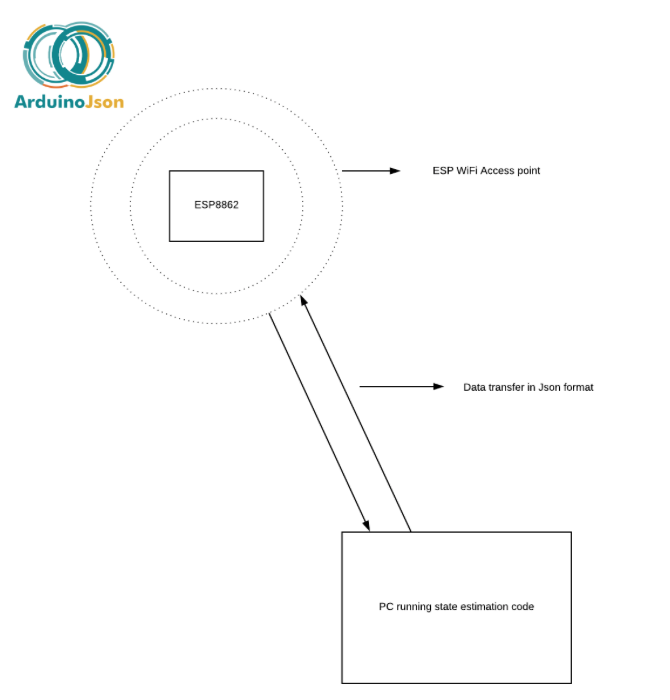
\includegraphics[width=110mm]{fig_3.png}
\caption{Communication diagram}
\label{fig:figure3}
\end{figure}

\newpage
\section{Motion Planning}
\subsection{Introduction}
In Lab 4, the two wheel robot car will perform parallel parking between two rectangular shape obstacles. First the ideal behavior of the car was simulated in Matlab and then implemented on the car.
In the simulation, assumption was the obstacles are located at right top corner and left top corner of the box and the car would start somewhere in the left half space of the box(Figure 4).

\begin{figure}[h!]
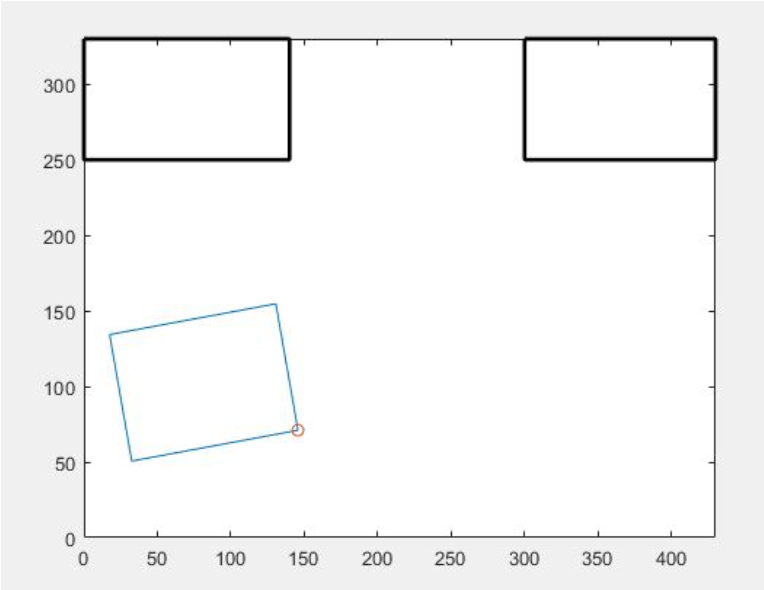
\includegraphics[width=110mm]{fig_4.png}
\caption{Position of the robot and obstacles}
\label{fig:figure4}
\end{figure}

As shown in the figure, the origin coordinates are set to be the left bottom corner. The measurement scale is 1mm. The obstacles are marked as the black bordered rectangles and the blue one is the car. The small red circle at right front corner of the car is where the range sensors are placed.  
In this set up, the motion planning algorithm then calculates an optimal path for the car to 
successfully finish its parallel parking
without hitting the obstacles or the walls.

\newpage 
\section{Algorithm}
This section goes the implemented algorithm in this lab. The motion planning procedure applied consists of two main functions : 
\begin{itemize}
	\item Get Milestones
	\item Get Control Inputs 
\end{itemize}

\subsection{Get Milestones}
This function, as the name suggests, finds a series of milestone positions that the car must reach on its way the destination.
In the very beginning of the function, all the required constants and dimensions are input which then will be used to calculate the milestones(Figure 5). These constants are previously defined in page 4 "Symbols" section. 
\\
\begin{figure}[h!]
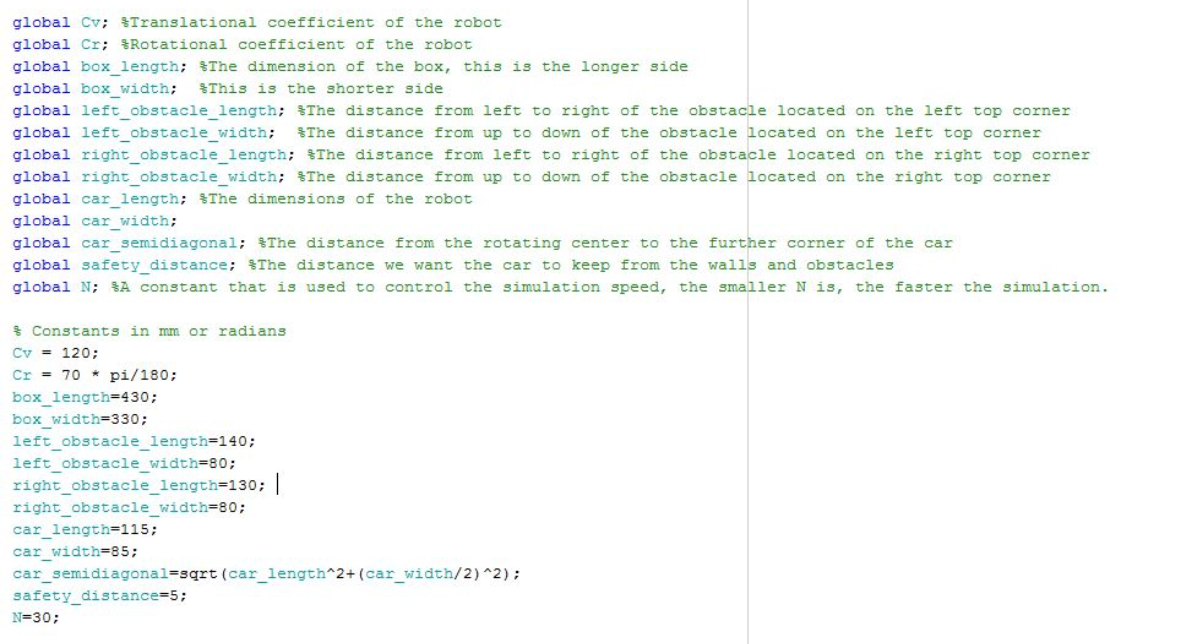
\includegraphics[width=110mm]{fig_5.png}
\caption{Get Milestoens function initialization}
\label{fig:figure5}
\end{figure}

The "safety" constant initialized in the code is used to create a range of safe distance shield around obstacles and the walls so the car moving in the box would not hit any of them. 

\begin{figure}[h!]
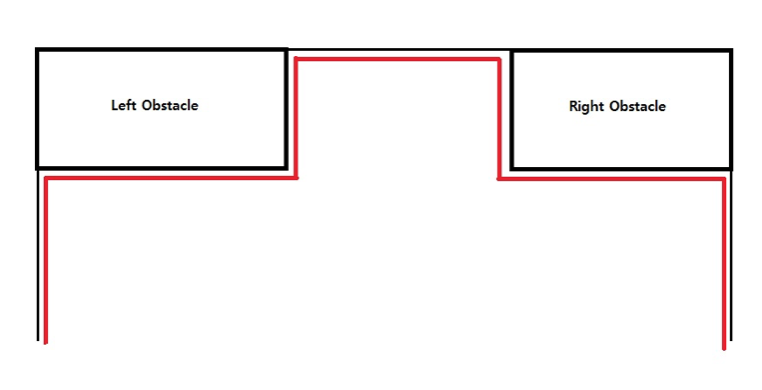
\includegraphics[width=110mm]{fig_6.png}
\caption{Indication of the safety distance around obstacles and the walls}
\label{fig:figure6}	
\end{figure}

\newpage
Safety distance for the code shown in Figure-5 is set
to be equal to 5, which means the car would always keep
a 5 millimeter distance from the obstacles and walls.
The corresponding distance is measured as the gap
between the red line and black lines in Figure-6.

\begin{figure}[h!]
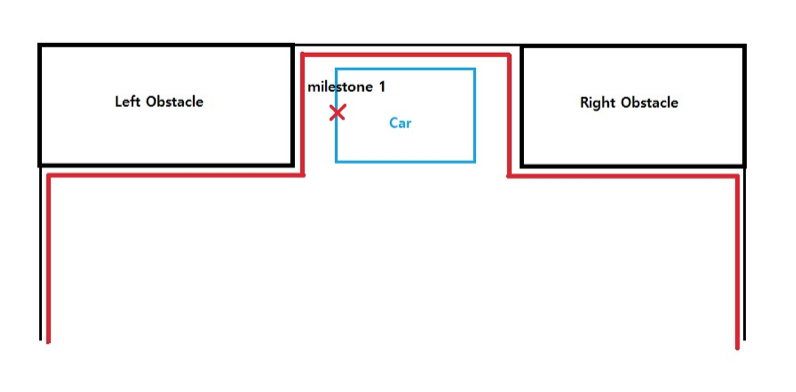
\includegraphics[width=110mm]{fig_7.png}
\caption{Finding the first Milestone}
\label{fig:figure7}	
\end{figure}

Then the function will find the first milestone position such that when the rotating center(the middle point of the segment that connects the centers of two wheels) of the car reach that position, the car will be the same distance away from both obstacles.(Figure 7)
This milestone 1 is what we call the destination milestone. In other words, if the car successfully gets to this position, the parallel parking is completed.

\begin{figure}[h!]
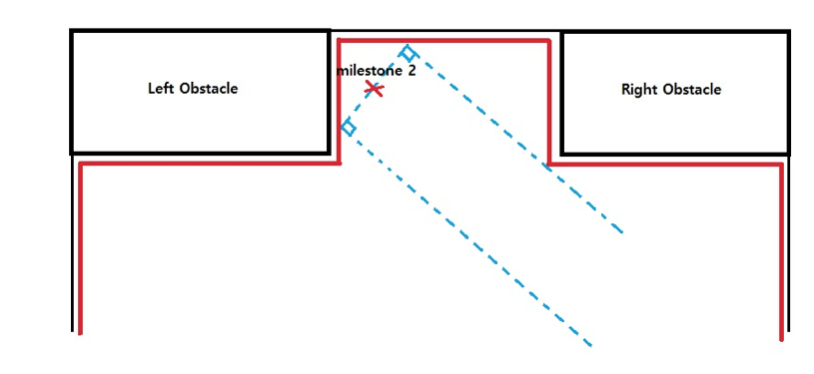
\includegraphics[width=110mm]{fig_8.png}
\caption{Finding the first Milestone}
\label{fig:figure8}	
\end{figure}

The next step is to find the milestone position that the car must reach before getting into the parking space, where the car starts to back up somewhere close to the right obstacle.
Seemingly, the milestone 2 might look very close to the milestone 1 in this specific case when the parking space is pretty narrow. 
Unlike Milestone 1 that can be directly found by looking at the dimensions of the objects,milestone 2 has to be derived from solving the equation shown in next figure.
\newpage
\begin{figure}[h!]
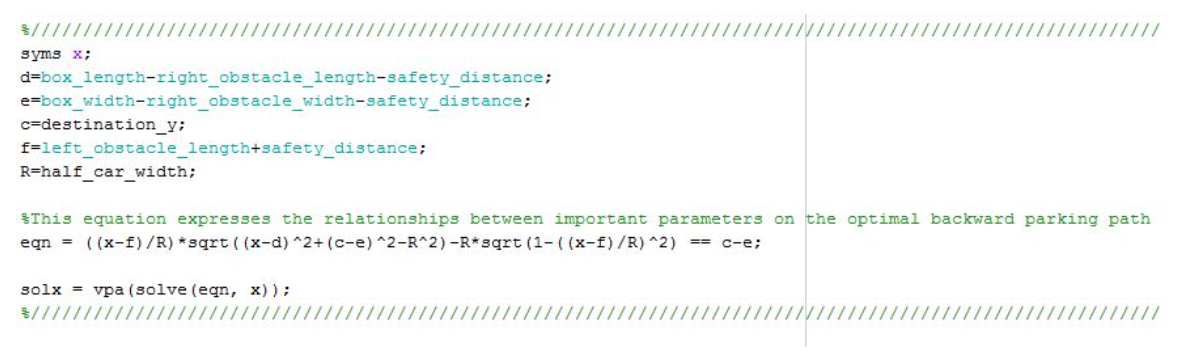
\includegraphics[width=110mm]{fig_9.png}
\caption{Deriving Milestone 2 position}
\label{fig:figure9}	
\end{figure}

Figure 6 shows the equation we used to find the x 
coordinate of the milestone 2. The equation describes 
the geometric surrounding of the parking space and the
relationships between important constant parameters.
This equation will guarantee that the car won’t hit any
of the obstacles or the wall while it is moving backward into the parking space and eventually rotate to face the obstacle.
As it can be seen in Figure 6, all of the parameters 
are defined by the global constants. So if we change 
the settings for any of the objects, this equation will 
change accordingly, and gives out different answer.
This way the algorithm can be utilized on any different set of box and obstacles as long as the constants and global variables modified accordingly. 
The milestone 2 is the most important milestone in the algorithm. Once this milestone calculated, the rest of the milestones are easier to be calculated. 

\begin{figure}[h!]
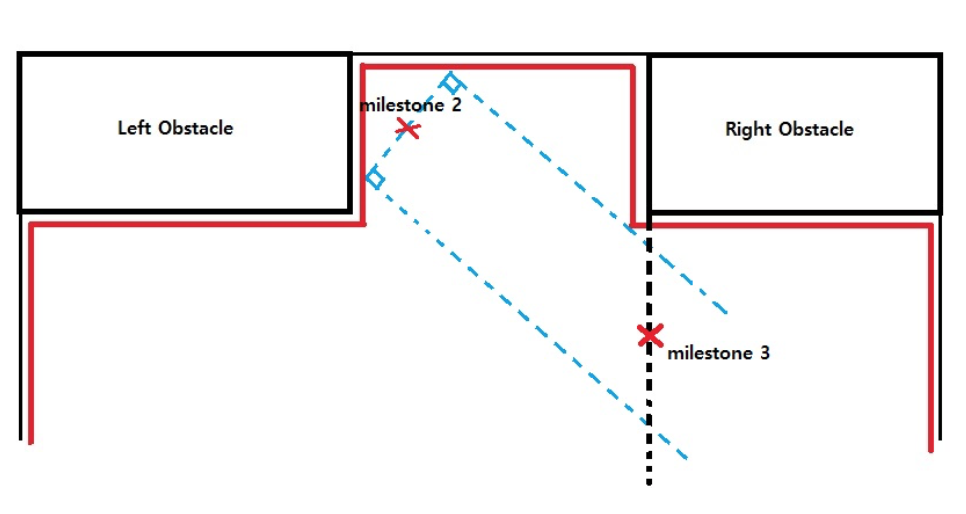
\includegraphics[width=110mm]{fig_10.png}
\caption{Deriving Milestone 3 position}
\label{fig:figure10}	
\end{figure}

The milestone 3 is the position that the car must reach right before starting to move into the parking space. It can be found based on the coordinates of the milestone 2. 
Draw the expected trajectory of the car(blue dash line) and then the black dash line by extending the left boundary of the right obstacle. The intersection of these two lines is what will be used to calculate milestone 3. 
\newpage
\begin{figure}[h!]
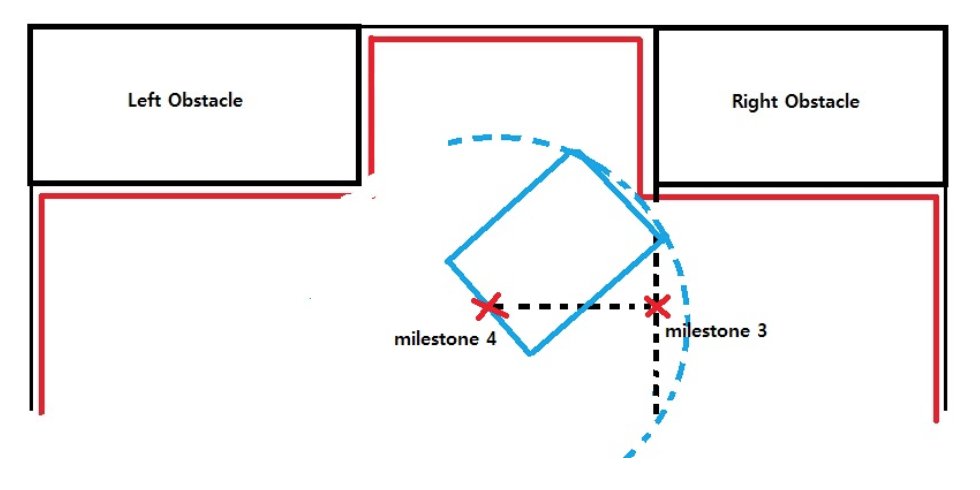
\includegraphics[width=110mm]{fig_11.png}
\caption{Deriving Milestone 4 position}
\label{fig:figure11}	
\end{figure}

To find the milestone 4, the function will first make a horizontal line that starts from the milestone 3 to the left. 
Then it will try to make a circle that has the center on the drawn line with the radius of the “semi-diagonal” of the car and check if the circle has any intersections with the red line.(red line being the defined safety distance)
It will define the center of the circle as the milestone 4 when the circle is tangent with the red line corner of the right obstacle.
The “Get Milestones” will then, finally, output these four milestone coordinates so that the “Get Control Inputs” function can use them as its guidance to generate the proper control inputs for the car.

\begin{figure}[h!]
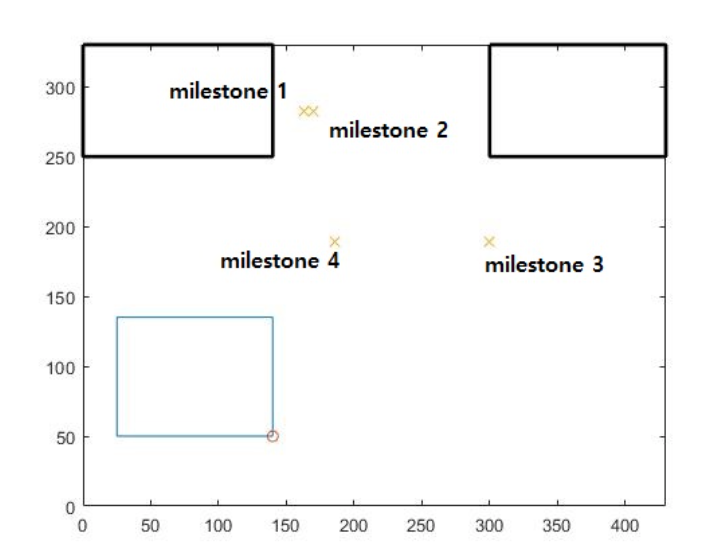
\includegraphics[width=110mm]{fig_12.png}
\caption{All Milestones overview}
\label{fig:figure12}	
\end{figure}

The actual result from calling the “Get Milestones” is the shown in figure 12. 

\newpage

\subsection{Get Control Inputs}
Running "Get Milestones" gives the positions the car needs to visit in order to perfom the parallel parking.  
Now calling "Get Control Inputs" will generate 3 required control inputs in order to move the car in the right path considering milestones.  
These 3 inputs are sorted as :  “turn, move, turn”. Meaning, the first input tells the car to turn a certain degree and the second input tells the car to move by a certain distance, and the last input tells the car to turn by another certain degree.
\linebreak
Now, suppose we initially put the car at the position  shown in Figure 12, calling the “Get Control Inputs” function we will generate the following inputs.(Figure10)

\begin{figure}[h!]
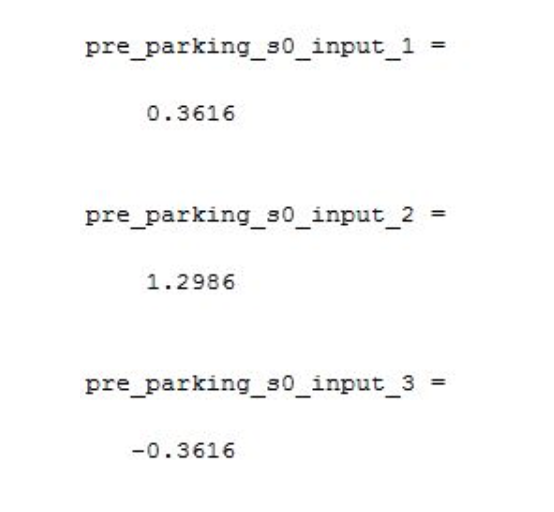
\includegraphics[width=110mm]{fig_13.png}
\caption{"Get Control Inputs" function call}
\label{fig:figure13}	
\end{figure}

If we check Figure 5, there are two constants $Cv=120$ 
and $Cr=70$. (Defined in "Symbols" section 1)
\\These are the transnational and the rotational constant of the car. It means, given  
$input=1$ the car will move by 120 millimeter or rotate by about 70 degrees. 
Considering these two constants and if we look at Figure 13, we can see that 
the 3 inputs will do “turning the car counter clock 
wise by $70 \times 0.3616$ $^{\circ}$, move the car forward by 
$120 \times 1.2986 mm$ and turn the car clock wise by $70 \times 0.3616$ $^{\circ}$. 
\newpage

\begin{figure}[h!]
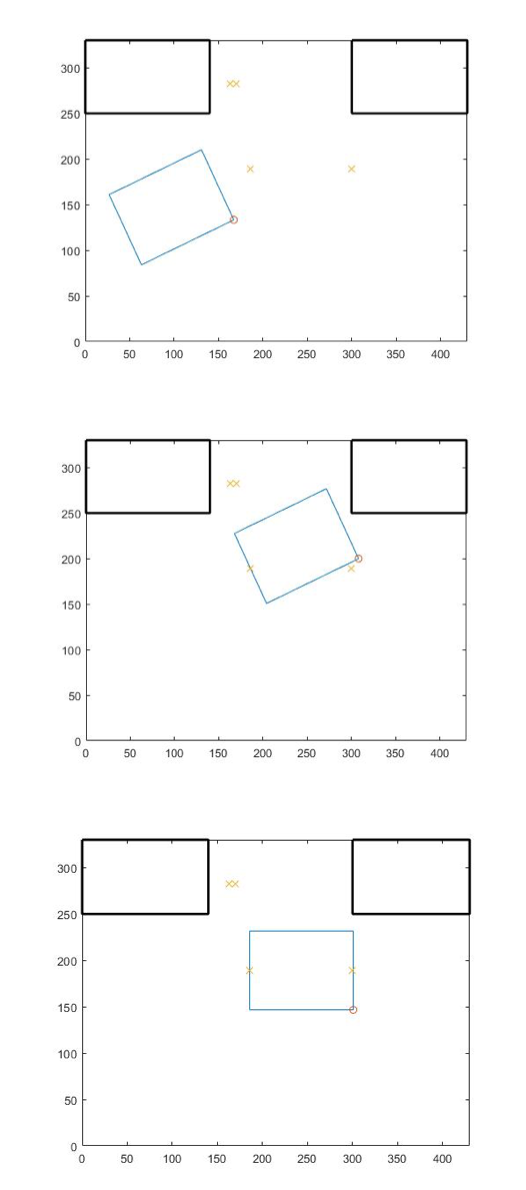
\includegraphics[width=70mm]{fig_14.png}
\caption{sequential motion commands}
\label{fig:figure14}	
\end{figure}

The first picture in Figure 14 shows the result after 
plugging the first turning input, the second picture 
shows the result after plugging the moving input, the 
last picture is the result after plugging the second 
turning input.
Similarly, when the function has been noticed that the 
car has reached the target milestone, it will generate 
the next series of inputs to lead the car to the next 
milestone position and it continues the same procedure   until the car gets to the destination milestone to complete its parallel parking (Figure 15).
\newpage
For more about the dynamic Matlab simulation of our algorithm please check the “Dynamic Simulation” folder on our GitHub page.
(Link given in References) 
\\ Below is the result of running the complete simulation in Matlab.  

\begin{figure}[h!]
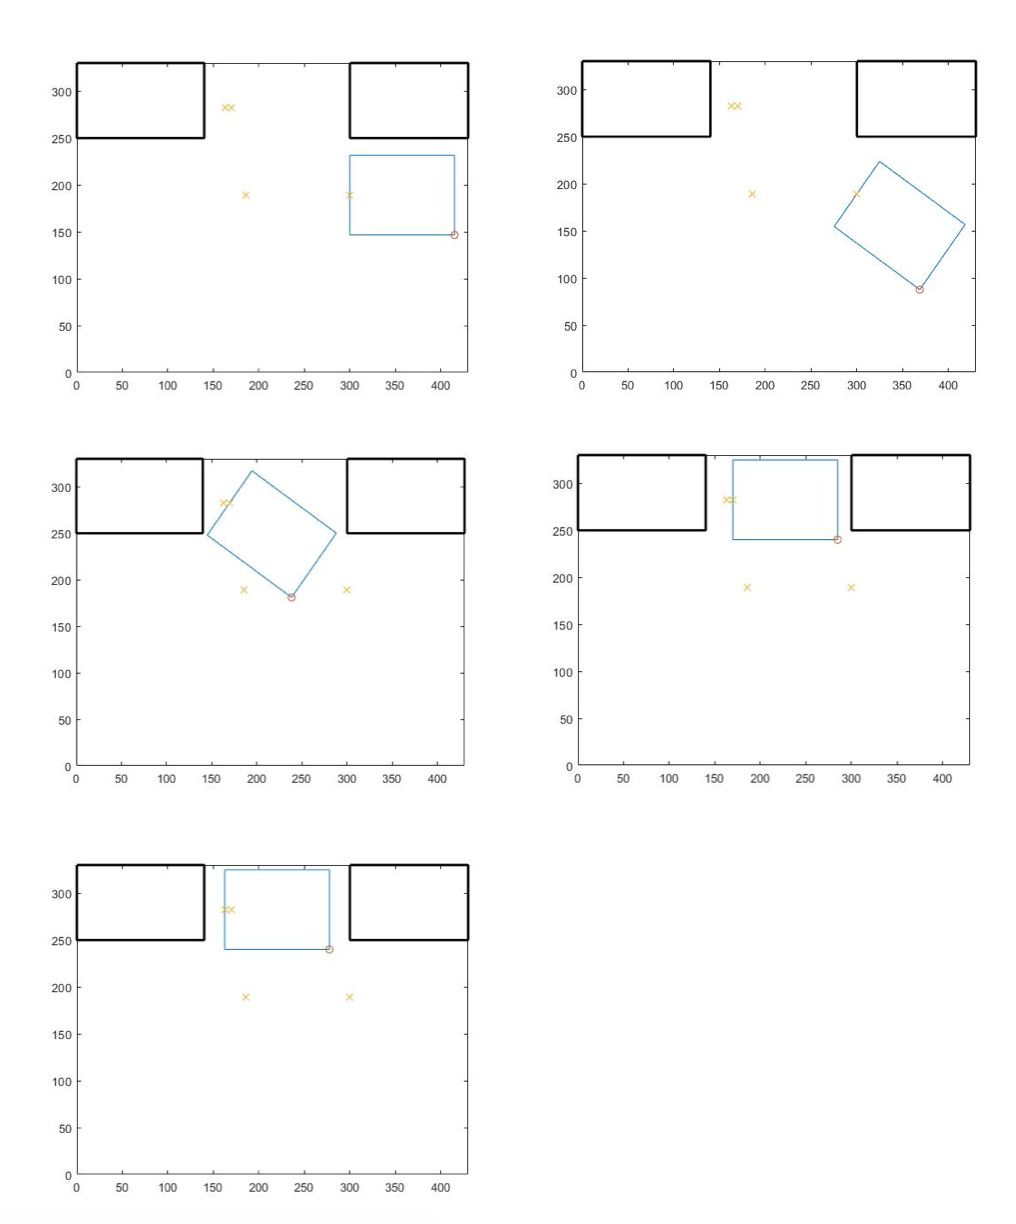
\includegraphics[width=110mm]{fig_15.png}
\caption{Complete Parallel Parking Process}
\label{fig:figure15}	
\end{figure}
\newpage
\section{Results}
For testing the algorithm on the actual module we got help from the state estimation Kalman filter derived in lab 3. 
In additoin to Kalman filter, we added two more variables to improve the performance of the car, which are the “acceptable radius” and “Close Enough”.(Figure 16)
\begin{figure}[h!]
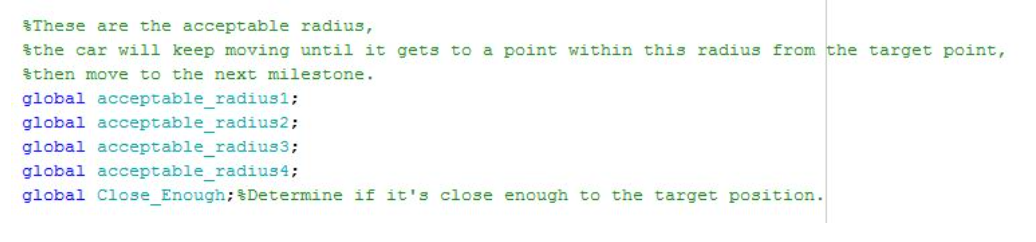
\includegraphics[width=110mm]{fig_16.png}
\caption{Motion Planning Helper variables}
\label{fig:figure16}	
\end{figure}

For example, assuming $set acceptable_radius1=10$ if then the car gets to a position that is within 
10mm from the first milestone, it will consider it
as “close enough” to the target.
\\ The "Close Enough" boolean variable will be set to 1 if the distance is within defined range,it will otherwise be set to 0. This 
variable is used to determine if the car is close 
enough to the current target milestone so that it can 
start moving to the next milestone in the next step.

\begin{figure}[h!]
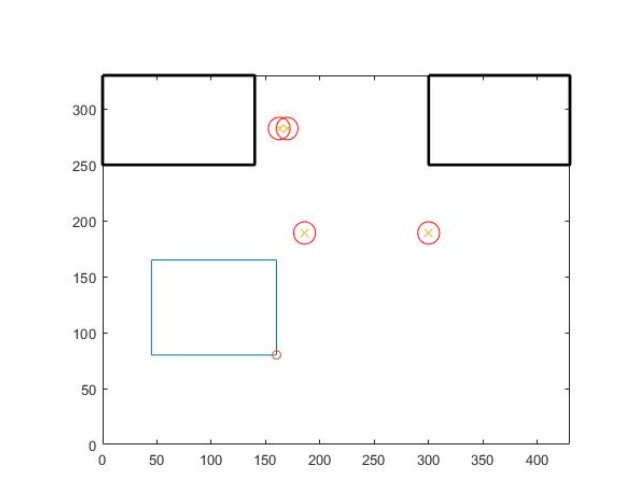
\includegraphics[width=110mm]{fig_17.png}
\caption{acceptable radius variables for different milestones}
\label{fig:figure17}	
\end{figure}
\newpage
In the main control code, we put a “while” statement (Figure 18) for each of the milestone points. Inside the loop, 
the “Get Control Inputs” function will keep generating 
the inputs to order the car to get closer and closer to 
the target spot until the car is distanced within,
specified range, from the milestone. Therefore the
variable “Close Enough” is set to 1.

\begin{figure}[h!]
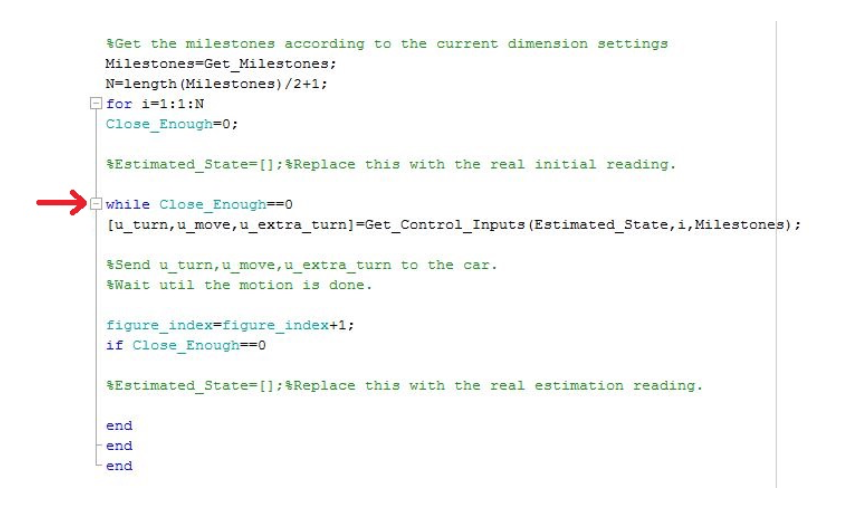
\includegraphics[width=110mm]{fig_18.png}
\caption{while loop statement for control system}
\label{fig:figure18}	
\end{figure}


As it can be seen in Figure 18, the new inputs are 
recalculated in the iteration loops based on the 
current estimated states. 
If the estimated states are reliable and the process 
errors are decently small, we can expect this 
algorithm to give a pretty good result on the real 
world parallel parking. And it indeed did a good job in 
our actual tests.
In our real world parking experiments, we have recorded 
the expected positions and the estimated positions 
around all of the milestone points and plotted them as 
figures when the parking is finished. Figure 19 shows 
the result of one the run tests we did. For more information about the real time tests, please refer to section 11 ("Demonstrations").

\begin{figure}[h!]
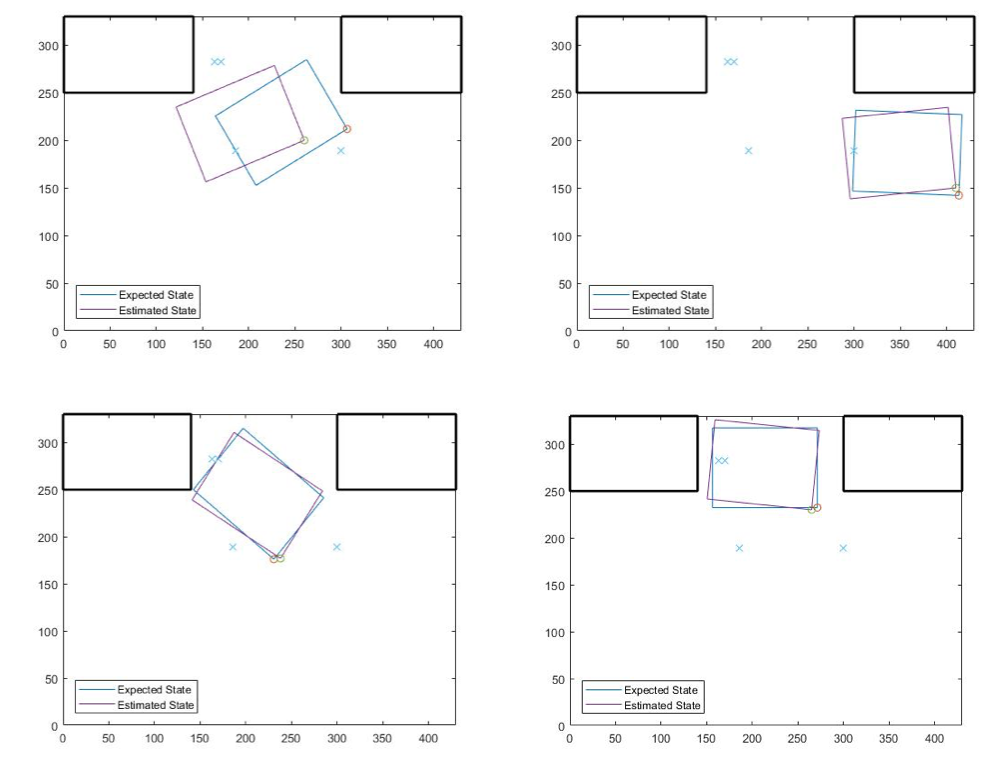
\includegraphics[width=110mm]{fig_19.png}
\caption{Real time simulation, Results recorded in Matlab}
\label{fig:figure19}	
\end{figure}
\newpage

\section{Demonstration}
All codes and related documents are uploaded to Github: 
\\
\url{http://google.com}
\\For demonstration videos please visit links below:
\begin{itemize}
\item Full demo (motion planning and state estmiation combined) \\
\url{https://youtu.be/30bCeLLuHEQ}
\item State Estimation Demo 
\url{https://youtu.be/0avIQL3_okI}
\item Motion Planning Demo test case 1
\url{https://youtu.be/0AI09jDCzT4}
\item Motion Planning Demo test case 2 
\url{https://youtu.be/vqe-3CE-YhE}
\item Motion Planning Demo test case 3 
\url{https://youtu.be/mMm7KnLYAuQ}
\item Motion Planning Demo test case 4 
\url{https://youtu.be/OZEuJw4zu0I}
\end{itemize}


 
\end{document}

%==================================================%
% Bibliography starts here
%==================================================%
% \bibliographystyle{unsrt}
% \bibliography{my_latex_math_template}

%%% Local Variables:
%%% mode: latex
%%% TeX-master: t
%%% End:
